%!TEX program = xelatex
%!TEX TS-program = xelatex
%!TEX encoding = UTF-8 Unicode
\let\nofiles\relax

\documentclass[algorithmlist, AutoFakeBold, AutoFakeSlant, figurelist, tablelist, nomlist, masters]{seuthesix}
\usepackage{xeCJK}
\usepackage{fontspec, xltxtra, xunicode}
\usepackage{graphicx, subfig}
\usepackage{autobreak}
\usepackage{amsmath, amssymb}
\usepackage{tabularx, array, multirow}
\usepackage{float}
\usepackage{algpseudocode}
\usepackage{booktabs}
\usepackage{enumerate}
\usepackage{longtable}
\usepackage{algorithm}
\usepackage{algorithmicx}
\usepackage{algpseudocode}
\usepackage{bm}
\usepackage{longtable}
\usepackage{enumitem}
\usepackage{natbib}


\renewcommand{\algorithmicrequire}{ \textbf{Input:}} %Use Input in the format of Algorithm
\renewcommand{\algorithmicensure}{ \textbf{Output:}} %UseOutput in the format of Algorithm


\XeTeXlinebreaklocale “zh” 
\XeTeXlinebreakskip = 0pt plus 1pt minus 0.1pt %文章内中文自动换行
%公式编号设置
% \numberwithin{equation}{section}
% % \makeatletter
% % \@addtoreset{equation}{section}
% % \makeatother
\renewcommand\theequation{\arabic{chapter}-\arabic{equation}}

\makeatletter
\newenvironment{breakablealgorithm}
  {% \begin{breakablealgorithm}
    \begin{center}
      \refstepcounter{algorithm}% New algorithm
      \hrule height.8pt depth0pt \kern2pt% \@fs@pre for \@fs@ruled
      \renewcommand{\caption}[2][\relax]{% Make a new \caption
        {\raggedright\textbf{\ALG@name~\thealgorithm} ##2\par}%
        \ifx\relax##1\relax % #1 is \relax
          \addcontentsline{loa}{algorithm}{\protect\numberline{\thealgorithm}##2}%
        \else % #1 is not \relax
          \addcontentsline{loa}{algorithm}{\protect\numberline{\thealgorithm}##1}%
        \fi
        \kern2pt\hrule\kern2pt
      }
  }{% \end{breakablealgorithm}
    \kern2pt\hrule\relax% \@fs@post for \@fs@ruled
    \end{center}
  }
\makeatother

\setcitestyle{comma}
\setlength{\bibsep}{1.5pt}
\setenumerate[1]{itemsep=0pt,partopsep=0pt,parsep=\parskip,topsep=5pt}
\setitemize[1]{itemsep=0pt,partopsep=0pt,parsep=\parskip,topsep=5pt}
\setdescription{itemsep=0pt,partopsep=0pt,parsep=\parskip,topsep=5pt}
% 表题 图题 章节号连接符
\renewcommand {\thetable} {\thechapter{}-\arabic{table}}
\renewcommand {\thefigure} {\thechapter{}-\arabic{figure}}
\begin{document}
\captionsetup{labelformat=default, labelsep=space}

% \bibliographystyle{seuthesix}
\setcounter{secnumdepth}{4}
\setcounter{tocdepth}{4}
\newtheorem{definition}{定义}[chapter]
\newcommand{\tabincell}[2]{\begin{tabular}{@{}#1@{}}#2\end{tabular}}  

\categorynumber{TP18} % 分类采用《中国图书资料分类法》
\UDC{004.8}            %《国际十进分类法UDC》的类号
\secretlevel{公开}    %学位论文密级分为"公开"、"内部"、"秘密"和"机密"四种
\studentid{201965 }   %学号要完整,前面的零不能省略。
\title{基于知识图谱表示学习的知识推理方法研究}{}{Research on Knowledge Reasoning Methods based on Knowledge Graph Representation Learning}{}
\author{周星辰}{Xingchen Zhou}
\advisor{汪鹏}{}{Peng Wang}{Associate Prof.}
% 空白的时候需要加转移符
% \advisor{\  }{\  }{ \ }{\  } 
% \coadvisor{楚留香}{副教授}{Perfume Tsu}{Associate Prof.} % 没有% 可以不填
\degreetype{工程硕士}{Master of Engineering} % 详细学位名称
\major{计算机技术}
\submajor{}
\defenddate{}
\authorizedate{\ }
\committeechair{}
\reviewer{}{}
\department{东南大学计算机科学与工程学院}{School of Computer Science and Engineering}
\makebigcover
\makecover

\begin{abstract}{表示学习,知识推理,强化学习,知识图谱}
我是一个人。
\end{abstract}

\begin{englishabstract}{represent learning, knowledge reasoning, reinforcement learning, knowledge graph}
I am a human.
\end{englishabstract} 

\tableofcontents
\mainmatter  % 该命令切换到正文状态。页码从阿拉伯数字 1 开始,此前页码为罗马数字形式。

\chapter{绪论}
\section{研究背景}
知识图谱(Knowledge Graph, KG)最早由Google公司在2012年提出,用于将事实知识进行结构化处理,并将其应用于智能搜索引擎~\cite{singhal_2012}。Google 知识图谱的成功应用,引起了学术界和工业界的广泛关注。知识图谱本质上是结构化的语义知识库,能够解释现实世界中的概念及关系~\cite{nickel2015review}。同时,知识图谱不采用诸如框架和脚本等繁琐的结构,而是采用形式更为灵活简单的<头实体,关系,尾实体>三元组以及与实体和关系相关的属性。其中,实体可以是现实世界的对象和抽象的概念,关系是实体之间的联系,实体和关系具有相应的属性。为了更直观地展示和分析知识图谱,还可以将知识图谱中的实体和关系分别作为节点和边,采用网络图的形式表示知识图谱~\cite{noy2019industry}。随着智能信息化的不断发展,知识图谱已被广泛应用于数据检索~\cite{rinaldi2021semantic,sarhan2021open,li2021research}、智能问答~\cite{li2021improving,do2021developing}、大数据分析决策~\cite{zhou2021geoscience,abu2021relational}等领域。典型的知识图谱如图~\ref{background_KG}所示,其中包含各种类型的实体和关系信息,同时实体之间存在概念层次结构。

\begin{figure}
  \centering
  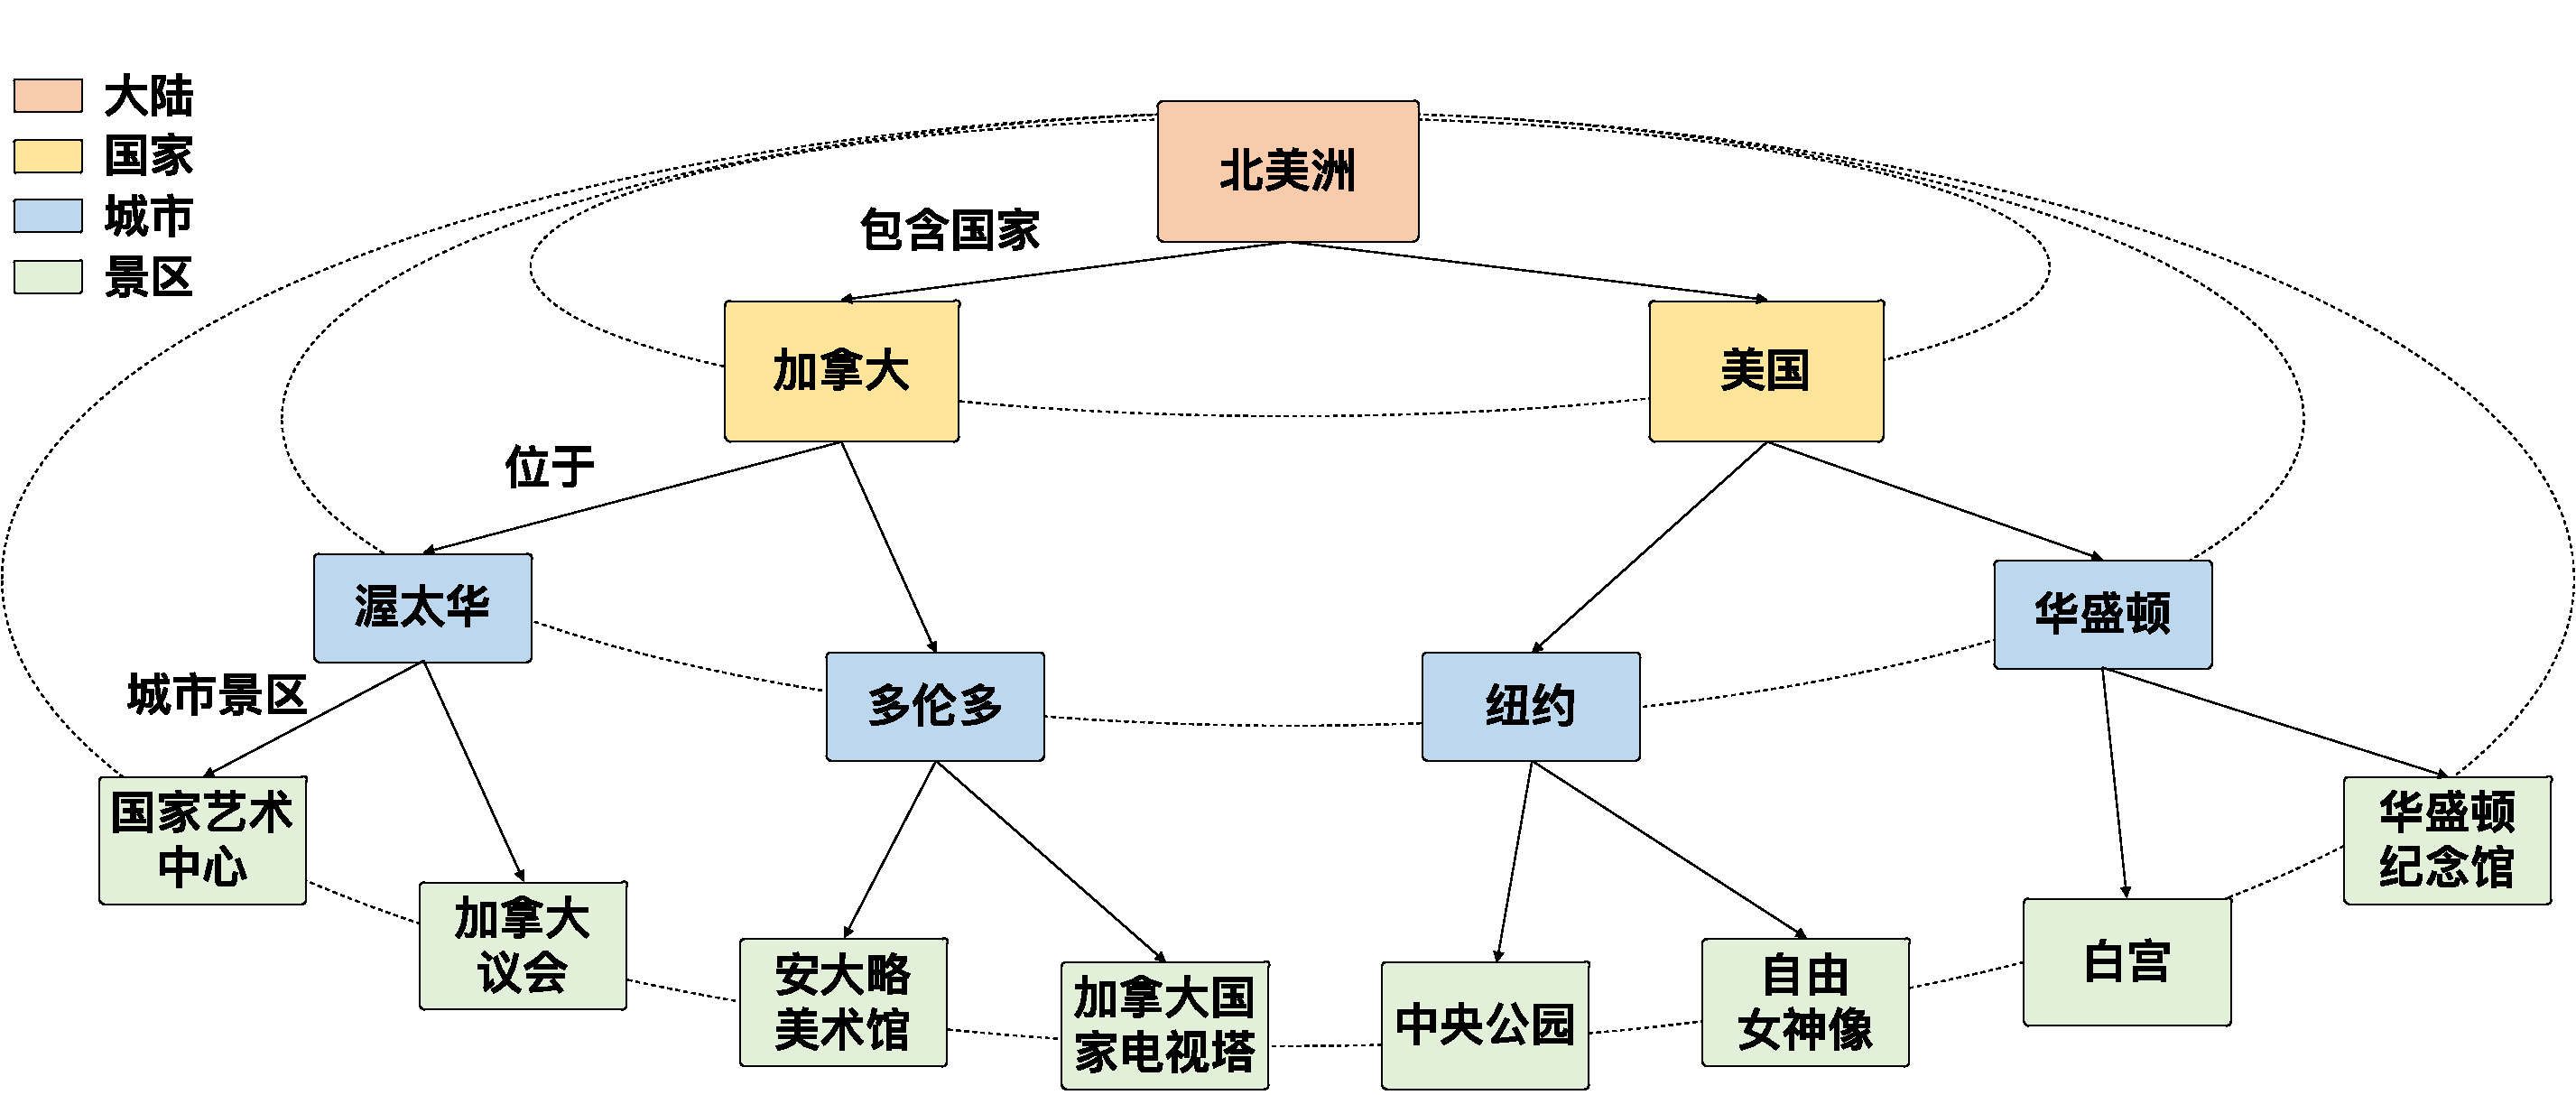
\includegraphics[width=0.9\textwidth]{1_KG}
  \caption{知识图谱}
  \label{background_KG}
\end{figure}

在实践中,知识图谱旨在作为组织或社区内不断发展的知识共享基础。知识图谱可以分为两类,分别是通用知识图谱和领域知识图谱~\cite{hogan2021knowledge}。两类知识图谱的原理相同,区别在于知识范围和应用领域,两种知识图谱在国内外均已得到广泛应用。国外的通用知识图谱包括百科知识图谱Freebase~\cite{bollacker2007platform},DBpedia~\cite{lehmann2015dbpedia}和Yago~\cite{hoffart2011yago2},多语言百科知识图谱Wikidata~\cite{vrandevcic2014wikidata},词典知识图谱WordNet~\cite{miller2007wordnet}和常识知识图谱CYC~\cite{lenat1995cyc}等。国内的通用知识图谱则包括中文百科知识图谱Zhishi.me~\cite{niu2011zhishi},该知识图谱首先采用固定的抽取规则,从百度百科、互动百科和中文维基百科中抽取实体信息,随后对不同百科的实体进行对齐,从而完成实体链接。CN-DBpedia~\cite{xu2017cn}是复旦大学开发的大规模通用领域结构化百科,从中文百科类网站的纯文本信息中提取信息,经过过滤、融合、推断等步骤后构成高质量结构化数据。领域知识图谱主要服务于特定行业领域,随着知识图谱在工业界的推广,逐渐发挥着越来越重要的作用。国外的领域知识图谱包括服务网络搜索的Google~\cite{singhal_2012}知识图谱,服务社交网络的LinkedIn~\cite{Qi_2016}知识图谱,服务商业领域的Aribnb~\cite{Spencer_2018}和Amazon~\cite{Krishnan_2018}知识图谱,以及服务金融领域的Banca d’Italia~\cite{bellomarini2019knowledge}知识图谱等。国内的领域知识图谱包括百度~\cite{wang2013xlore}、淘宝~\cite{xu2021alime}、微博~\cite{wei2020analysis}等企业的知识图谱。由于领域知识图谱涉及到具体而复杂的领域场景,需要业务和开发专家的配合,因此对领域知识图谱的设计和开发提出了更高的要求。

知识图谱能够采用简洁的表示形式,将复杂多样的知识转化为清晰的三元组形式,并提供了强大的知识存储和推理能力。然而,知识图谱的知识信息通常采用自然语言进行描述,难以被计算机所处理和应用。因此,为了方便知识图谱的后续应用,需要将知识图谱内的知识信息转换为计算机能够直接处理的向量形式,这项技术被称为知识图谱表示学习(Knowledge Representation Learning, KRL)~\cite{chen2022rlpath}或知识图谱嵌入(Knowledge Graph Embedding, KGE)~\cite{wang2021transet}。知识图谱表示学习模型能够将知识图谱中的实体和关系映射到低维稠密的向量空间进行表示,同时保留其中的结构和语义信息,从而能够进行知识推理等知识应用工作。知识图谱表示学习主要涉及四个问题:(1)选择何种表示空间:现有的模型采用的表示空间可以分为欧几里得空间~\cite{lu2022dense}、流形空间~\cite{ebisu2018toruse}、复向量空间~\cite{trouillon2016complex}和黎曼空间~\cite{pan2021hyperbolic}。(2)采用何种评分函数:现有的评分函数包括基于距离的评分函数~\cite{sachan2020knowledge}和基于语义相似度的评分函数~\cite{xiao2017ssp}。(3)应用何种编码模型:现有模型采用的编码模型包括线性模型~\cite{peng2020lineare}、双线性模型~\cite{pan2021hyperbolic}、因式分解模型~\cite{ji2015knowledge}和神经网络模型~\cite{jiang2021kernel}。(4)是否采用辅助信息,以及采用何种辅助信息:可以加入文本信息、视觉信息和类型信息等多种辅助信息~\cite{wang2017knowledge}。通过知识图谱表示学习,可以将知识信息转换为向量表示,作为知识补全等下游任务的输入。由于知识图谱通常是采用自动或半自动的方式进行构建,因此通常是不完整的。通过现有知识预测知识图谱中缺失的知识,进行知识图谱补全,是提高知识图谱质量的有效手段~\cite{vu2019capsule}。

知识图谱的典型应用中包括知识图谱补全和知识图谱问答。尽管知识图谱表示学习能够完成部分知识图谱补全和知识图谱问答的工作,但无法对关系路径进行建模,而只能基于单个实体或者关系进行简单的补全或问答。同时,知识图谱表示学习通过向量计算的方法进行隐式的知识补全,本质上属于黑盒模型,无法提供充分的证据,可解释性比较差。因此,需要借助知识图谱上的知识推理方法,综合考虑知识图谱网络图的拓扑结构信息,对复杂关系路径进行建模,从而解决更为复杂的知识图谱补全和知识图谱问答内容,并提供相应推理证据~\cite{chen2020review}。知识推理不局限于传统的基于逻辑的和规则的推理方法,还可以采用更多样化的推理方法,随着知识图谱表示学习等技术的发展,一系列新的知识推理方法不断涌现,例如随机游走方法~\cite{jagvaral2020path}、路径排序方法~\cite{zhao2021target}、启发式方法~\cite{he2021heuristic}和神经网络方法~\cite{wang2018deep}等。丰富的知识图谱内容为知识推理技术的发展提供了新的机遇和挑战。

综上所述,知识图谱在人工智能应用中具有较大价值,基于知识图谱的知识图谱表示学习有助于将知识图谱转化成易于处理和应用的知识图谱表示向量,并为下游任务提供充分的支持。知识推理是知识图谱智能应用的一个重要任务,深入研究该任务,有助于加深对知识图谱的认知,并充分和有效地利用知识图谱的知识。因此,本文旨在提出一种有效的知识图谱表示学习模型,随后基于知识图谱表示学习模型,实现一种知识推理模型,在适用于大规模知识图谱的前提下,同时保证知识推理的质量,并能够解决多种推理任务。

\section{研究现状}
\subsection{知识图谱表示学习研究现状}
知识图谱能够有效地表示知识图谱中的结构化数据,但是难以被计算机进行直接处理和应用,需要先通过知识图谱表示学习的过程将知识三元组转换为向量的形式,才能应用于各类知识图谱推理任务。知识图谱可以表示为$G=\{E, R, F\}$,其中$E$、$R$和$F$分别表示实体、关系和事实的集合。知识图谱内的事实三元组可以表示为$(h, r, t) \in F$,其中$h$、$r$和$t$分别表示头实体、关系和尾实体。例如,对于给定的事实三元组$\left(\mbox{美国,首都,华盛顿特区}\right)$,其中的$\mbox{美国}$是头实体$h$,$\mbox{华盛顿特区}$是尾实体t,$\mbox{首都}$则是头实体和尾实体之间的关系$r$。同时根据定义,有$h \in E$,$t \in E$,以及$r \in R$。经过知识图谱表示学习后,可以将知识图谱中的节点和关系映射到低维稠密向量空间中。使用粗体字符表示知识图谱表示向量,则完成知识表示后的三元组为$\left(\bm{h}, \bm{r}, \bm{t}\right) \in \mathbb{R}^{\mathrm{d}}$,这里设置向量空间为$d$维的欧几里得空间,也可以投影到其他类型的向量空间。为了构建知识图谱表示学习模型,需要完成三个步骤:(1)定义实体和关系在向量空间的表示形式。在这一步中,需要选择向量空间,设计编码模型,并确定是否需要辅助信息。(2)定义评分函数$f_r(h, t)$,用于评价事实$\left(\bm{h}, \bm{r}, \bm{t}\right) \in \mathbb{R}^{\mathrm{d}}$的合理性。知识图谱中可见事实三元组的得分一般会高于潜在事实三元组的得分。以及(3)学习实体和关系的表示,使知识图谱中可见事实三元组的总置信度最大化。

目前的知识图谱表示学习模型可以分为翻译模型,语义匹配模型和因果推断模型。

\subsubsection{翻译模型}
翻译模型采用基于距离的评分函数,将关系看做头实体和尾实体之间的翻译,并将关系翻译后两个实体之间的距离作为得分,进而实现衡量事实三元组的合理性。

翻译模型的典型代表是Bordes等人提出的TransE模型~\cite{bordes2013translating},其思想源于Mikolov等人提出的词嵌入模型word2vec~\cite{toms2013},在该模型中发现了词向量空间中存在平移不变性,例如。TransE将知识图谱中的实体和关系映射到$d$维欧几里得空间中,即$\left(\bm{h}, \bm{r}, \bm{t}\right) \in \mathbb{R}^{\mathrm{d}}$,并将关系看做是实体之间的连接向量,遵循$\bm{h} + \bm{r} \approx \bm{t}$,例如$\bm{h}\left(\mbox{美国}\right) + \bm{r}\left(\mbox{首都}\right) \approx \bm{t}\left(\mbox{华盛顿特区}\right)$。同时对于给定三元组$\left(h, r, t\right)$,通过计算向量$\bm{h} + \bm{r}$和$\bm{t}$之间的$L1$或$L2$距离,进而得到三元组的合理性得分。对于较为合理的三元组,其得分应尽量接近0,对于不合理的三元组,则希望其得分相对较高。TransE模型采用的得分函数可以表示为:$f_r(h, t) = \|\bm{h} + \bm{r} - \bm{t}\|_{\ell_1 / \ell_2}$。尽管TransE模型在大规模知识图谱表示学习方面取得了巨大进步,但在处理如一对多、多对一和多对多等复杂关系时仍然存在困难。例如,给定两个三元组$\left(\mbox{北京,所属国家,中国}\right)$和$\left(\mbox{上海,所属国家,中国}\right)$,其中是多对一类型的关系,根据TransE模型的要求$\bm{h} + \bm{r} \approx \bm{t}$,则实体$\mbox{北京}$和$\mbox{上海}$会被映射到向量表示空间中十分接近的位置。然而这两个实体实际上存在较大差异,因而这种映射是不合理的。

为了更好地处理复杂关系问题,Wang等人提出的TransH模型~\cite{wang2014knowledge}扩展了原始的TransE模型,为每种关系分别构建关系超平面,从而让一个实体在不同的关系超平面中会得到不同的表示向量。对于关系$r$,TransH会采用关系$r$独有的平移向量$d_r$和超平面法线向量$w_r$对关系进行表示。对于给定三元组$\left(h, r, t\right)$,TransH首先将$h$和$t$的表示向量沿着法线向量$w_r$的方向映射到关系超平面,设$h_\perp$和$t_\perp$分别为头实体和尾实体的映射向量,则有$\bm{h}_{\perp} = \bm{h} - \bm{w}_r^{\top} \bm{h} \bm{w}_r$,$\bm{t}_{\perp} = \bm{t} - \bm{w}_r^{\top} \bm{t} \bm{w}_r$。随后用关系平移向量$d_r$连接头实体向量和尾实体向量。TransH模型的评分函数为$f_r(h, t) = \left\|\bm{h}_{\perp} + \bm{d}_r - \boldsymbol{t}_{\perp}\right\|_2^2$。虽然TransH模型使得实体能够根据关系获得不同表示,但全部实体和关系仍然在分布在相同的特征空间$\mathbb{R}^{\mathrm{d}}$中。由于实体具有多种语义,而不同关系可能关注实体的不同语义,因此单个特征空间可能不足以反映实体和关系的这一性质。

为了解决上述问题,Lin等人提出的TransR~\cite{lin2015learning}进一步扩展了TransH,将关系超平面扩展到了关系空间,即为每种关系构建对应的关系空间。对于给定三元组$\left(h, r, t\right)$,TransR将实体$h$和$t$映射到实体向量空间$\mathbb{R}^{\mathrm{d}}$中,同时为每个关系设置了相应的投影矩阵$\mathbf{M_r} \in \mathbb{R}^\mathrm{k \times d}$,能够将实体向量映射到关系$r$对应的向量空间$\mathbb{R}^{\mathrm{k}}$。设$\bm{h_\perp}$和$\bm{t_\perp}$分别为头实体和尾实体的映射向量,则有$\bm{h}_{\perp}=\bm{M}_r \bm{h}$,$\bm{t}_{\perp} = \bm{M}_r \bm{t}$。TransR采用投影矩阵,因此时空复杂度高于TransE和TransH。Ji等人提出的TransD~\cite{ji2015knowledge}模型很好地改善了TransR模型存在的问题。TransD对给定三元组$\left(h, r, t\right)$中每个实体和关系都构建两组向量,其中一组向量用来表示实体或关系的含义信息,表示为$\bm{h, t} \in \mathbb{R}^{\mathrm{d}}$和$\bm{r} \in \mathbb{R}^{\mathrm{k}}$,另一个向量用于形成两个动态投影矩阵,表示为$\bm{h_p, t_p} \in \mathbb{R}^{\mathrm{d}}$和$\bm{r_p} \in \mathbb{R}^{\mathrm{k}}$。相应地,构建的动态投影矩阵为$\mathbf{M}_{r h} = \bm{r}_p \bm{h}_p^{\top} + \mathbf{I}$,$\mathbf{M}_{r t}=\bm{r}_p \bm{t}_p^{\top} + \mathbf{I}$,其中$\mathbf{I}^{\mathrm{k \times d}}$是单位矩阵。设$\bm{h_\perp}$和$\bm{t_\perp}$分别为头实体和尾实体的映射向量,则有$\bm{h}_{\perp}=\mathbf{M}_{r h} \bm{h}$,$\bm{t}_{\perp}=\mathbf{M}_{r t} \bm{t}$。通过构建动态投影矩阵,TransD降低了矩阵运算的时空复杂度。

上述模型主要目标在于通过改变实体和关系的表示空间,提高表示学习的效果。除此之外,还有一些研究者从评分函数和编码方式的角度入手改进模型。对于给定的三元组$\left(h, r, t\right)$,TransM~\cite{fan2014transition}将与关系相应的权重$\theta_r$相关联,并将评分函数定义为$f_r(h, t)=-\theta_r\|\bm{h} + \bm{r} - \bm{t}\|_{1 / 2}$。通过给一对多、多对一和多对多关系分配较低的权重,可以让向量$\bm{h} + \bm{r}$和$\bm{t}$之间留有更大的距离。MainfoldE~\cite{xiao2016one}将$\bm{h} + \bm{r} \approx \bm{t}$的要求弱化为$\|\bm{h} + \bm{d} - \bm{t}\|_2^2 \approx \theta_r^2$,从而将$t$映射到以$\bm{h} + \bm{r}$为中心,半径为$\theta_r$的超球体,而不再是靠近$\bm{h} + \bm{r}$的确切点。同时,MainfoldE的评分函数定义为$f_r(h, t) = -\left(\|\bm{h} + \bm{r} - \bm{t}\|_2^2 - \theta_r^2\right)^2$。TransA~\cite{xiao2015transa}在TransR的基础上,使用自适应马氏距离代替传统的欧氏距离,并定义评分函数为$f_r(h, t) = -(|\bm{h} + \bm{r} - \bm{t}|)^{\top} \mathbf{M}_r(|\bm{h} + \bm{r} - \bm{t}|)$,从而使模型在处理复杂关系时更加灵活。

\subsubsection{语义匹配模型}
语义匹配模型采用基于相似度的评分函数,通过分析实体和关系的向量空间表示捕获语义信息,进而评估事实的合理性。模型的核心方法是,首先将知识图谱中的事实三元组$\left(h, r, t\right)$转换为三维的二元张量$\mathbf{X} \in \mathbb{R}^{\mathrm{n \times n \times m}}$,其中n为实体数量,m为关系数量,张量的每个切片$\mathbf{X_k}(k=1,2, \ldots, m)$对应相应的关系,张量值$\mathbf{X_{i j k}}$代表事实三元组$\left(h_i, r_j, t_k\right)$是否存在于知识图谱中,如果为1则存在,为0则不存在。

RESCAL~\cite{nickel2011three}是语义匹配模型的典型代表,采用张量来表示知识图谱的结构。对于关系$r_k$,有张量切片$\mathbf{X_k} \approx \mathbf{A R_k A^{\top}}$,其中矩阵$\mathbf{A}$用于捕获实体的潜在语义表示,矩阵$\mathbf{R_k}$用于对头尾实体对的交互进行建模。对于给定的三元组$\left(h, r, t\right)$,RESCAL的评分函数定义为$f_r(h, t)=\bm{h}^{\top} \mathbf{M}_r \bm{t}$,其中$\bm{h}, \bm{t} \in \mathbb{R}^d$是实体的嵌入向量,$\bm{M}_{\bm{r}} \in \mathbb{R}^\mathrm{d \times d}$表示关系中的潜在语义信息。通过张量分解的方法,RESCAL能够较好地捕获实体和关系的语义信息,并给出三元组的合理性得分。然而,RESCAL的计算复杂度比较高。为了改善模型的时空复杂度,DistMult~\cite{yang2015embedding}将$\mathbf{M_r}$限制为对角矩阵,即$\mathbf{M}_r=\operatorname{diag}(\bm{r}), \bm{r} \in \mathbb{R}^\mathrm{d}$。随后,评分函数被调整为$f_r(h, t)=\bm{h}^{\top} \operatorname{diag}(\bm{r}) \bm{t}$。通过这样的转换,DistMult显著降低了算法复杂度,同时在实验结果上取得了提高。然而,DistMult对头实体和尾实体的计算是对称的。对此,ComplEx~\cite{trouillon2016complex}模型通过复数嵌入,能够在不对称关系中扩展DistMult模型。实体和关系被嵌入到了复数空间$\mathbb{C}^\mathrm{d}$中,同时评分函数被修改为$f_r(h, t)=\operatorname{Re}\left(\bm{h}^{\top} \operatorname{diag}(\bm{r}) \bar{t}\right)$,其中$\operatorname{Re}(\cdot)$表示复数值的实数部分,$\bar{t}$表示尾实体的复数共轭部分。通过该评分函数,具有不对称关系的三元组就可以根据实体的序列获取不同的分数。

另一种具有代表性的语义匹配模型是RotatE~\cite{sun2018rotate}。受欧拉恒等式$e^{i \theta}=\cos \theta + i \sin \theta$的启发,RotatE引入了旋转哈达玛积,它将关系视为复数空间中头实体到尾实体的旋转,对于给定的三元组$\left(h, r, t\right)$,RotatE的评分函数为$f_r(h, t) = \|\bm{h} \circ \bm{r} - \bm{t}\|$,其中$\circ$表示旋转哈达玛积。通过这种方式,RotatE具有较好地表示和推理能力,能够处理对称/反对称关系、自反关系和复合关系。然而,RotatE采用的旋转哈达玛积在处理部分三元组时存在局限性。例如,给定三元组$\mbox{母亲,父亲,祖母}$和$\mbox{父亲,母亲,祖父}$,RotatE计算时会判断$\mbox{父亲的母亲}$与$\mbox{母亲的父亲}$是逻辑等价的,并将$\mbox{祖母}$和$\mbox{祖父}$映射到向量空间中角度接近的位置,但这种推导显然是错误的。为了解决这一问题,QuatE~\cite{zhang2019quaternion}模型将RotatE从复数空间扩展到四维空间,并采用哈密尔顿积替换旋转哈达玛积,用于捕获实体和关系间的潜在语义关联。相应的评分函数为$f_r(h, t)=\bm{h} \otimes \bm{r}|\bm{r}|^{-1} \cdot \bm{t}$,其中$\otimes$表示哈密尔顿积。由于哈密尔顿积的前后算子不可交换,所以能够区分类似$父亲的母亲$和$母亲的父亲$这样的实体概念,从而较好地解决RotatE存在的问题。

\subsubsection{因果推断模型}
因果推断模型将因果推断方法引入知识图谱表示学习领域,主要思想是引入因果干预方法,增强模型的领域适应性,减少局部结构差异,从而提高模型的泛化能力。同时通过因果分析还能够确定知识图谱表示学习时哪些特征信息有助于进行实体和关系表示,并提高相应的信息权重,进而增强模型的表示效果。

Wang等人提出的NIC模型~\cite{wang2021neighborhood}将因果推断模型与知识图谱表示学习领域相结合,提高了表示效果。知识图谱表示学习模型通过设计表示空间、评分函数和编码模型,并考虑加入辅助信息,完成模型的构建。对于给定的三元组$\left(h, r, t\right)$,模型会通过评分函数$f_r\left(h, t\right)$给出三元组的合理性评分。在训练模型学习实体和关系的向量表示时,通常选择优化目标是使得知识图谱中已有三元组的评分尽可能比未出现的三元组评分更高。然而,训练过程中的评分主要用于进行结果排序,而不是作为三元组的置信度得分。这导致评分函数的效果下降,限制了知识图谱补全等知识推理工作的发展。例如,给定三元组$\left(h, r, t\right)$,常规知识图谱表示学习方法的评分函数$f_r\left(h, t\right)$得到相应评分为0.9,但该三元组的实际置信度得分只有0.3,即评分与置信度得分存在不匹配的问题。因此,为了解决上述问题,使得评分函数能够给出接近实际置信度的评分,NIC提出了一个基于因果干预的置信度评估方法,称为邻里干预一致性(Neighborhood Intervention Consistency,NIC),通过验证预测结果的稳定性来评估置信度分数,具体方法是调整实体向量在不同维度上的值,设置为集合$\{0, \operatorname{avg}(\bm{e}), \max (\bm{e}), \min (\bm{e})\}$中的任意一种,即可以取零值、平均值、最大值和最小值其中之一。如果调整所有特征中的权值会导致时间效率过低,因此NIC通过特征选择获取不同维度的贡献,贡献计算函数为$w_j=|E|^{-1} \sum_{i=0}^{|E|}\left(\mathbf{E}_{i, j}-\operatorname{avg}\left(\mathbf{E}_{:, j}\right)\right)^2$,并选择贡献最大的维度进行调整。完成调整后,观察模型的输出序列是否改变或者是否与原始序列匹配,匹配度计算方法为$\zeta\left(S, S^{N_i}\right)=\sum_{j=0}^J \sigma(S)_j\left(1-\operatorname{Sgn}\left(\left|\varrho(S)_j-\varrho\left(S^{N_i}\right)_j\right|\right)\right)$,其中$\sigma$和$\operatorname{Sgn}$分别为Softmax函数和Sign函数,该函数可以表示因果干预后预测结果的稳健性。随后给出置信度得分为$p_{n i c}(S)=d^{-1} \sum_{i=0}^d\left(\varsigma\left(S, S^{N_i}\right)\right)$,为0到1之间的实数。

另一种具有代表性的因果推断知识图谱表示学习模型为Feng等人提出的CGI模型~\cite{feng2021should},采用图卷积神经网络。图卷积神经网络广泛应用于知识图谱表示学习中,其主要思想是通过聚合实体节点的邻域信息实现实体表示效果的增强。然而,由于知识图谱中局部结构属性存在较大差异,即存在局部结构差异问题,从而造成实体节点表示存在不一致分布的问题,这导致对不同节点使用相同的聚合方法会降低节点表示效果。通常的解决方案是采用注意力机制,通过训练降低可能导致局部结构差异的邻居的权重,然而通常无法实现理想情况的注意力机制效果。针对上述问题,CGI采用了因果图卷积神经网络模型,该模型能够根据局部结构的因果效应调整训练好的图卷积神经网络模型。CGI首先得到节点的原始表示向量,该向量受到邻域特征和自身特征的影响。随后采用因果干预,将邻域置位空,从而实现屏蔽图结构,并要求实体节点根据自身特征获取表示向量。因果干预过程可以表示为$e=f(x, \mathcal{N}(x) \mid \theta)-f(x, \operatorname{do}(N=\emptyset) \mid \theta)$,其中$\operatorname{do}(N=\emptyset)$表示执行因果干预,将邻域置为空集合。最后CGI根据局部结构的因果效应、预测置信度和其他因素,采用一个独立的二元分类器$D=\{(x, p) \mid \hat{z}=z \cup \hat{z}=z\}, p=\operatorname{flag}(\hat{z}=z)$,在因果干预表示和原始表示之间进行选择。实验证明模型通常能够在遇到局部结构差异时选择因果干预表示,即屏蔽邻域特征仅采用节点自身特征的表示。

\subsection{知识推理研究现状}
通过知识图谱表示学习模型可以通过链接预测的方式实现知识推理,即给定查询三元组$\left(h, r, ?\right)$,$\left(h, ?, t\right)$或$\left(?, r, t\right)$,通过将知识图谱内所有关系或实体作为候选答案,输入到知识图谱表示学习模型中,从而将实体与关系映射到低维向量空间中,并通过得分函数进行打分,随后根据得分结果进行排序,选择得分最高的实体或关系作为答案,并完成知识推理。然而,基于知识表示学习模型的推理在形式上只能完成单跳的推理,无法显式地进行多跳推理,因而无法提供推理路径。这使得推理过程缺乏可解释性~\cite{wang2019deeppath}。为了解决这一问题,提出了关系路径推理方法,该类方法利用知识图谱上的拓扑结构信息,在知识图谱的关系路径上进行建模和推理。采用关系路径推理的方式,不仅可以得到推理结果,同时还可以给出一个可解释的路径指示推理过程。

现有的知识推理模型可以分为符号逻辑推理模型,神经推理模型和神经符号推理模型。

\subsubsection{符号推理模型}
符号推理模型(Symbolic reasoning model)旨在为非结构化自然语言查询语句生成结构化的查询。现有的符号推理模型可以分为语义解析和基于模板的知识推理两种方法。其中,语义解析方法通过自然语言处理工具,将问题转换为句法依赖表示。基于模板的知识推理方法则构建大量模板,包括自然语言模式和相应的结构化查询模式(例如SPARQL),从而实现复杂问题的分解。

马尔科夫符号网络(Markov Logic Network, MLN)~\cite{richardson2006markov}是基于预定义的规则和知识图谱中的事实三元组信息构建的概率图模型,能够在模型训练的过程中学习不同规则的权重,最终。具体而言,给定一个具体的规则集合,其中的每个规则都可以通过知识三元组进行具体查询,则可以通过下列步骤完成MLN模型的构建:首先为每个规则对应的知识三元组构建一个对应节点,如果知识三元组存在则节点值设为1,否则设为0。随后如果两个节点如果对应同一个规则,则在两个节点之间构建一条边。最后令每个规则对应一个特征,如果规则成立则特征值为1,否则特征值为0。规则的所有节点都共享这个特征。完成MLN模型构建后,网络中所有节点的联合分布定义为$P(X=x)=Z^{-1} \exp \left(\sum_i w_i n_i(x)\right)$,其中$w_i$是对应规则的权重,是$n_i$规则对应节点的数量。随后可以通过MCMC算法进行MLN模型的推理,并通过优化伪似然度量实现权重的学习。基于学习的权重,即可以完成具体的路径推理。通过引入权重信息,MLN能够较好地将一阶谓词逻辑和概率图模型进行结合,并实现不确定性的推理。然而,知识图谱结构十分复杂,造成了MLN的推理非常困难且效率低下。此外,知识图谱中缺失的三元组也会影响规则推理的效果。为了解决上述问题,pLogicNet~\cite{qu2019probabilistic}综合了MLN和图嵌入技术的思想,首先通过MLN定义知识图谱中事实三元组的联合分布,并对每种逻辑规则与权重构建关联,随后采用变分EM算法有效地学习权重。在EM算法中,E步骤推断未观察到的三元组的合理性,其对应的变分分布采用TransE等知识图谱表示学习模型进行参数化,M步通过优化观察到的三元组和知识图谱表示学习模型得到的三元组上的伪似然来更新逻辑规则的权重。通过上述方法,pLogicNet可以实现高效知识推理,同时能够处理知识图谱中缺失的信息。

另一类符号逻辑推理模型的代表是ProbLog~\cite{de2007problog},它是逻辑编程语言ProLog的一个改进。ProLog能够基于给定规则、事实和查询语句进行自动的知识推理并给出答案。ProbLog则是对于每种规则设置了一个概率,并令最终的知识推理给出推理的概率,从而模拟知识推理过程中的不确定性。给定查询,则推理概率被定义为$P\left(q \mid T\right)=\sum_{L \in L_T} P(q, L \mid T)$,其中T描述了原因L的概率分布,因此推理概率被分解为查询的所有联合概率和每种可能的原因集合的总和。其中有$P(q, L \mid T)=P(q \mid L) \cdot P(L \mid T)$,进一步分解了推理概率,其中$P(L \mid T)$表示给定原因的情况下查询的概率,如果至少有一个答案能够使查询为真,则对应的$P(L \mid T)$的值为1。式中另一项,即原因集合的概率的计算方法为$P(L \mid T)=\prod_{c_i \in L} p_i \prod_{c_i \in L_r \backslash L}\left(1-p_i\right)$。为了计算$P(L \mid T)$,一种方法是枚举所有可能的逻辑规则和对应的事实,效率较低。另一种方法是采用ProLog的选择线性确定(Selective Linear Definite,SLD)方案,采用自上而下的方式构造SLD树。首先通过查询步骤初始化根节点,随后通过应用每个规则及对应的事实来递归创建子目标,到达结束条件时停止迭代,即找到了查询目标或到达了树的最大深度。同时,每种查询结果都与一系列带有概率的规则相关联。

\subsubsection{神经推理模型}
神经推理模型的推理方法是将知识图谱中的实体、关系和查询问题共同编码到相同的表示空间中,并在表示空间中进行知识推理。传统的基于距离和基于语义匹配的模型无法满足知识推理的要求,为了获得更加有效的实体和关系嵌入效果,神经推理模型引入了神经网络结构,用于知识图谱邻域信息的建模。神经推理模型与知识图谱表示学习模型比较相似,都是首先进行知识图谱表示,随后实现知识推理等任务,但不同在于,神经推理模型会将自然语言查询问题也编码到表示空间中,从而增强知识推理的效果。同时,神经推理模型能够处理单跳问答、多跳问答和复杂逻辑问答问题,而知识图谱表示学习模型通常只能处理单跳问答问题。

ConvE~\cite{dettmers2018convolutional}是第一种采用卷积神经网络的神经推理模型,首先将头实体和关系映射到向量空间,随后将向量转换成矩阵并进行拼接,输入到卷积层中。ConvE采用二维卷积捕获两个实体之间的特征交互信息,并通过卷积层和全连接层获取实体之间不同维度的局部信息,返回特征图张量。随后,将张量转化为向量,并投影到向量空间,最后通过计算与尾实体向量的内积,得到最终的合理性得分。其评分函数为$f_r\left(h, t\right)f(\operatorname{vec}(f([\bm{h} ; \bm{r}] * \omega)) \mathbf{W}) t$,其中$\omega$为卷积核,$\mathbf{W}$为权重矩阵。此外,ConvE还引入了一个一对多的评分程序,能够自动匹配所有尾实体,从而能够更有效率地评估所有候选答案尾实体。然而,ConvE将实体和关系向量转换为矩阵并进行拼接,这一过程丢失了翻译模型的平移不变性。对此,ConvKB~\cite{nguyen2018novel}去除了ConvE的转换操作,并采用一维卷积保持平移不变性,同时捕获实体之间的全局关系和平移特征。ConvKB将每个三元组$\left(h, r, t\right)$的d维度嵌入表示为一个三列的矩阵$(\bm{h}, \bm{r}, \bm{t}) \in \mathbb{R}^{\mathrm{d} \times 3}$,随后将矩阵输入到卷积层,其中提供许多相同维度的过滤器,能够提取三元组中相同维度特征之间的全局关系,并通过对矩阵的每行进行操作以获得不同的特征图,最后将这些特征图拼接成一个三元组特征向量,并通过和权重矩阵进行点积运算得到最终的三元组合理性得分,评分函数为$f_r(h, t)=\operatorname{concat}(g([\bm{h}, \bm{r}, \bm{t}] * \Omega)) \cdot \mathbf{W}$,其中$g$为激活函数,$\Omega$为过滤器,$\mathbf{W}$为权重矩阵。HypER~\cite{balazevic2019hypernetwork}是基于ConvE提出的又一种卷积神经网络推理模型,采用基于ConvE的超网络为每个关系生成卷积滤波器权重,超网络可以实现跨层的权重共享,并动态生成给定输入的权重。HypER使用基于特定关系的一维卷积滤波器来处理实体嵌入,这简化了嵌入模式。同时,HypER使用卷积算子实现头实体嵌入和一组特定于关系的滤波器$F_r$,滤波器是超网络$H$从关系嵌入中创建的,超网络的结构是一个全连接层。最后,HypER还应用了ReLU激活函数的权重矩阵$\mathbf{W}$实现特征图张量的向量化。HypER的评分函数为$f_r(h, t)=f\left(\operatorname{vec}\left(\bm{h} * F_r\right) \mathbf{W}\right) \bm{t}$,相较于ConvE,HypER具有更强的表达能力和更少的参数。

传统的神经推理模型通过单向关系路径或文本信息引入上下文信息,而忽略了实体之间的各种连接模式,以及不重要的路径和词的影响,这造成模型无法充分捕捉三元组之间的关系信息。为了解决这一问题,R-GCN~\cite{schlichtkrull2018modeling}采用关系图卷积网络,显式地对多关系知识图谱进行建模并捕获实体周围的单跳邻域事实信息。R-GCN由编码器和解码器构成,在对实体进行编码的时候,R-GCN能够综合考虑实体连接之间的各类输入和输出的关系信息,并对实体的结构信息进行充分的编码。实体表示被更新为$\bm{h}_i^{(l+1)}=\sigma\left(\sum_{r \in R} \sum_{j \in \mathbf{N}_i^r} c_{i, r}^{-1} \mathbf{W}_r^{(l)} \bm{h}_j^{(l)}+\mathbf{W}_0^{(l)} \bm{h}_i^{(l)}\right)$,其中$\mathbf{N}_i^r$是节点i在关系$r \in R$下的邻域,$c_{i,r}$是特定问题的归一化常数。解码时,可以通过基数分解和块对角矩阵分解的方法求解,并选择DistMult分解模型作为评分函数,认为每个关系都对应一个对角矩阵,从而得到最终的评分函数为$f_r(h, t)=\bm{h}^T \mathbf{R}_r \bm{t}$。R-GCN分析了知识图谱中邻域信息对实体表示的影响,但是没有显式地对实体间的关系进行建模。SACN~\cite{shang2019end}模型对R-GCN进行了改进,是一种加权的GCN模型,能够同时考虑节点间的连通性、节点的属性和关系类型。SACN同样由编码器和解码器构成。编码器部分,SCAN引入了不同类型关系的权重以对GCN模型进行改进,得到加权图神经网络。同时,在聚合信息时对不同类型的关系分别进行聚合,因此可以将多关系图按照多个单关系图的形式进行分析。此外,SACN还将实体属性作为属性节点加入到了实体表示部分,并采用类似的方法进行分析。在SACN模型中,实体表示被更新为$h_i^{l+1}\sigma\left(\sum_{j \in \mathbf{N}_i} \alpha_t^l \bm{h}_j^l \mathbf{W}^l+\bm{h}_i^l \mathbf{W}^l\right)$。解码器采用Conv-TransE进行解码,利用卷积过滤器直接对相同维度的实体和关系向量进行处理。

\subsubsection{神经符号推理模型}
神经符号推理模型(Neural-symbolic reasoning model)是符号推理模型和神经推理模型的结合,综合了两种模型的优点。现有的神经符号推理模型包括神经增强符号推理模型(Neural-enhanced symbolic reasoning model)和端到端推理模型。其中,神经增强符号推理模型仅仅用于将问题解析成结构化的查询,随后需要使用查询方法才能够得到最终答案。而端到端推理模型可以自动完成解析问题并检索答案的步骤。

DeepPath~\cite{wang2019deeppath}首先将强化学习模型应用到了关系路径知识推理方面,并开发了一种新的奖励函数,通过综合分析模型是否到达目标节点、模型推理路径长度是否过长和与已有路径嵌入向量的相似度,来提高准确性、路径多样性和推理效率。DeepPath首先采用翻译模型的方法,对连续空间中的代理状态信息进行编码,并选择知识图谱的关系空间作为强化学习模型的动作空间。另一种基于强化学习的模型是MINERVA~\cite{das2018go},根据基于LSTM的策略函数对邻域信息进行采样。同时,与DeepPath不同的是,MINERVA中的状态是由查询关系和部分路径的嵌入组成,在采样的过程中不需要答案实体的嵌入向量,从而能够允许MINERVA直接通过知识推理得到答案。同时,MINERVA还为知识图谱的每个节点增加了自关系,从而能够在推理过程中在到达答案实体时自动停止。然而DeepPath和MINERVA在分析模型是否到达目标节点时,提供的奖励机制比较简单,即如果代理到达目标节点则提供值为1的奖励,同时对没有达到目标节点的情况提供值为-1的惩罚或者值为0的奖励。这种方法导致了奖励稀疏问题并降低了模型探索路径的效果。对此,Multi-Hop模型~\cite{lin2018multi}改进了强化学习的奖励函数,将硬奖励替换成了基于真实答案实体和推理实体之间相似度的软奖励。同时,受到dropout技术的启发,Multi-Hop在模型训练的过程中丢弃了一些动作,从而避免选择大量重复路径,缓解过拟合问题。另一种缓解奖励稀疏的方法由M-Walk~\cite{shen2018m}模型提出,该模型采用了一种基于价值的强化学习方法,并使用蒙特卡洛树搜索(Monte Carlo Tree Search,MCTS)来客服奖励稀疏的问题。具体而言,M-Walk迭代地使用MCTS的轨迹生成步骤和策略改进步骤,实现细化策略函数,从而获得更多的奖励信息。

除去关系路径知识推理模型,另一种神经符号推理模型采用图结构进行推理。GraIL模型~\cite{teru2020inductive}采用图神经网络的形式,并在提取的子图上推理两个实体之间的关系。具体而言,GraIL首先提取头实体和尾实体周围的k跳子图并取交集,随后采用元组$(d(i, h), d(i, t))$标记子图中的实体,其中$i$表示子图中的第$i$个节点,$d$表示头实体和尾实体到节点的最短距离。随后采用基于注意力的多关系图神经网络,也就是R-GCN,计算每个节点的实体表示,最后将头实体、尾实体和查询关系的表示向量连接起来,并以此为基础在子图上进行推理。GraIL在学习与实体无关的关系语义方面具有很强的能力。CogGraph~\cite{du2019cognitive}从给定的头实体和查询关系开始,通过策略函数在每一步扩展多个实体,随后采用GNN模型获取节点在推理子图中的表示向量,并预测答案。DPMPN模型~\cite{xu2019dynamically}采用了两个图神经网络模型来执行推理。第一个模型在整个知识图谱上进行消息传递,用于提供实体表示。第二个模型在查询子图上修建消息传递图,用于捕获与查询相关的语义。

此外,还有基于矩阵的神经符号推理模型。这种模型可以看做图神经网络模型的扩展,其不会基于跳数选择邻居,而是综合软注意力分数来评估不同邻居的重要性。其基本思想是通过矩阵运算来表达头尾实体之间的重要性。TensorLog~\cite{cohen2016tensorlog}是较早提出的基于矩阵的模型,能够通过知识推理,得到带有权重的链式逻辑规则,从而解释知识图谱中的每个关系。随后基于推理得到的规则,输入头实体和关系,目标是通过检索对实体进行排名,将正确答案尽可能排在靠前的位置。TensorLog采用独热向量表示实体,并用矩阵表示知识图谱中的向量,其中如果知识存在于知识图谱中,则矩阵对应位置为1。但是,TensorLog中的参数较难学习,因为每种规则都对应一个参数,而枚举规则本身就是一个离散的任务。对此,神经逻辑编程(Neural LP)模型~\cite{yang2017differentiable}将规则的权重参数分解为了规则中谓词的权重。同时,设计了一个循环公式来动态建模规则的长度。最后,Neural LP计算所有向量的加权平均值,并使用注意力来控制规则的长度。上述两种方法可以学习一些概率链式逻辑规则,但是无法推断出一些复杂的规则形式,如树状规则。此外,链式规则是基于特定的头实体进行推断的,这也会降低学习的泛化性。对此,神经逻辑归纳学习(Neural Logic Inductive Learning, NLIL)模型~\cite{yang2019learn}将原始语句进行合并以处理非链式规则,并取得较好的效果。

\subsection{知识推理应用}
通过知识图谱表示学习模型,可以得到知识图谱内实体和关系的表示向量。随后通过知识推理模型,可以进一步利用知识表示向量内的信息,从而实现一系列知识推理应用。常见的知识推理应用主要包括知识图谱补全和知识图谱问答。

\subsubsection{知识图谱补全}
知识图谱补全(Knowledge Graph Completion,KGC)~\cite{vu2019capsule}指的是预测与实体有相应关系的实体的任务,即给定头实体$h$和关系$r$预测对应的尾实体$t$,或是给定关系$r$和尾实体$t$预测对应的头实体$h$,前者可以表示为查询三元组$\left(h, r, ?\right)$,后者可以表示为查询三元组$\left(?, r, t\right)$,这种类型的知识图谱补全任务被称为实体预测。类似的,另一种知识图谱补全任务是给定头实体$h$和尾实体$t$并预测关系$r$,可以表示为查询三元组$\left(h, ? t\right)$,这种知识图谱补全被称为关系预测。以查询尾实体为例,给定查询三元组$\left(h, r, ?\right)$,首先选择在知识图谱表示学习模型,将头实体$h$和关系$r$映射到向量空间中,随后可以选择将知识图谱中每个实体作为候选答案,并使用得分函数$f_r\left(h, t\right)$计算三元组得分。随后,将按照得分从高到低的顺序获取候选答案的有序序列,并检查正确答案在序列中的位置。评价知识图谱补全的好坏主要在于正确答案在最终候选答案序列中的位置是否靠前,通常采用的评价指标有平均排序MR(正确答案排名的平均值)、平均倒数排序MRR(正确答案排名倒数的平均值)以及Hits@K(正确答案在序列中排名位于前K的比例)等。

\subsubsection{知识图谱问答}
知识图谱问答(Knowledge Graph Question Answering,KGQA)包括单跳问答、多跳问答和复杂逻辑问答等多种形式~\cite{saxena2020improving}。其中,单跳问答与知识图谱补全类似,两者的区别在于,知识图谱补全采用查询三元组的形式,提供两个已知元素并要求模型通过推理得到未知的元素,从而实现知识图谱补全。知识图谱问答则不提供查询三元组,而提供自然语言查询语句$q$,并要求模型基于该问句进行问题的解答,答案类型可以是实体和关系。相比之下,多跳问答更加复杂,知识推理模型需要通过知识图谱上的多跳关键路径进行推理才能获得答案实体和关系,同时部分多跳问答数据集如HotpotQA还要求模型提供相应的证据来证明推理的有效性~\cite{yang2018hotpotqa}。复杂逻辑问答提供的查询语句中包含多个主题实体,主题实体之间通过连接词$\land$、析取词$\vee$和否定词$\neg$进行聚合,因此可以对每个主题词进行多跳推理,最后对推理结果进行求交集,获取最终答案。由于知识图谱问答采用自然语言问句进行查询,因此具有较高的难度。通常的解决方案是,首先对查询语句$q$进行实体识别,获取其中的主题实体,随后基于主题实体,可以采用知识图谱补全的方案,通过知识图谱表示学习模型进行单跳推理,或采用基于关系路径的知识推理模型进行多跳推理和复杂逻辑推理,最终得到目标实体或关系,实现问题求解。评价知识图谱问答的效果可以分析正确答案在最终答案候选序列的位置是否靠前,可以采用的评价指标有平均排序MR、平均倒数排序MRR和Hit@K等。

\subsection{存在问题分析}
随着DBpedia、Freebase和Yago等一系列大规模知识图谱的提出,知识图谱表示学习和知识推理的相关研究取得了重要进展。然而,尽管越来越多的知识图谱表示学习和知识推理模型在知识图谱补全和知识图谱问答等知识图谱应用中取得了瞩目的效果,但仍然面临着许多挑战:

\begin{itemize}
  \item [(1)]
  \textbf{知识图谱表示学习模型难以分析和体现知识的因果性}。现有的知识图谱表示学习模型通常直接选择捕获目标知识的相应实体和邻域中的信息进行表示学习,而没有进行因果分析和干预以避免局部结构差异。同时,评分函数给出的得分通常只用于排序,而不能反应知识的置信度,限制了模型在具体应用任务中的表现。
  \item [(2)]
  \textbf{知识图谱表示学习模型与知识推理模型的结合不够充分}。由于知识图谱表示学习模型与知识推理模型的训练过程相互分离,导致模型间的结合不够充分,从而降低了知识推理应用中的效果。
  \item [(3)]
  \textbf{知识推理模型的推理能力不足}。多跳推理任务在现实世界中十分常见,具有重要的研究和应用价值。然而现有的知识图谱推理模型对多跳推理的支持仍然较差,同时,采用知识图谱表示学习模型进行推理只能实现单跳推理,这限制了知识图谱表示学习模型在知识推理应用上的进一步应用。
  \item [(4)] 
  \textbf{模型可解释性较差}。采用神经网络结构的知识推理模型,由于模型结构可以理解为黑盒模型,所以难以分析模型得出结果的具体过程。同时,如果采用知识图谱表示学习模型直接进行知识推理,则模型只会得出推理结果,而不会提供相应的推理路径和证据信息,这导致难以分析模型推理的具体过程进而优化模型。
\end{itemize}

\section{论文工作}
当前知识图谱表示学习模型存在的问题包括:难以分析和体现知识的因果性,以及与知识推理模型的结合不够充分。同时当前知识推理模型存在的问题包括:知识推理模型推理能力不足和模型可解释性较差。
因此,针对现有知识图谱表示学习模型和知识推理模型存在的问题,本文提出了知识图谱表示学习模型NORMAN(k\textbf{NO}wledge graph \textbf{R}epresentation learning \textbf{M}odel based on c\textbf{A}usal i\textbf{N}ference),以及知识推理模型LAURA(know\textbf{L}edge graph re\textbf{A}soning model based on d\textbf{U}al-agent \textbf{R}einforcement le\textbf{A}rning)。
NORMAN模型首先获取知识图谱中的层次信息和知识表示向量,随后将它们作为输入提供给图神经网络模型进行模型训练,并在训练过程中将因果推断方法融入信息传递过程中以提高模型的稳定性,最终完成知识图谱表示学习模型的训练,得到的模型能够将知识转换为向量表示。
LAURA模型利用NORMAN模型提供的层次信息和知识表示向量作为输入,训练实体级和层次级两种粒度的强化学习推理模型,并通过协作策略网络和轨迹相似度奖励实现上述两种推理模型的信息交互合作,最终完成知识图谱推理模型的训练,得到的模型可以根据给定知识信息进行推理,返回知识推理路径和对应置信度信息。

本文的整体技术路线图如图XXX所示。从整体来看,本文首先需要研究层次性知识图谱,本文的主要工作包括:

\begin{itemize}
  \item [(1)]
  \textbf{提出一种基于因果推断的知识图谱表示学习模型},包含层次信息提取模块、因果推断模块和图神经网络模块。
  层次信息提取模块的目标是增强模型对层次信息的利用能力,提高模型对知识信息的表示效果。本文采用极坐标表示法,将知识映射到极坐标系中,并以半径坐标作为知识的层次信息,角坐标则用于区分相同层次的知识。通过对半径坐标进行聚类,可以实现对知识的层次信息提取,为因果推断模块提供数据支持。
  因果推断模块能够将因果推断融入知识图谱表示学习中,评估邻域信息是否有助于进行表示和推理并进行取舍。本文采用邻域信息因果干预的方法,综合考虑因果不确定性、预测置信度和层次类别信息等多种因素,判断当前节点是否接收来自邻域节点的信息。本文通过加入因果推断方法,提高知识图谱表示效果,为后续推理提供充分支持。
  图神经网络模块采用图神经网络模型,采用知识图谱中各个实体的邻域结构信息构建图神经网络模型,并通过知识邻域间的信息传递进行数据更新。在此过程中,模块利用层次信息提取模块的层次信息作为辅助,采用因果推断模块评估是否接收邻域信息。完成训练后的模型,能够将输入的知识结构化三元组转换为表示向量,并可以用于后续知识推理工作。
  \item [(2)]
  \textbf{提出一种基于双重代理强化学习的知识推理模型},包含实体级强化学习模块、层次级强化学习模块和双重代理强化学习交互模块。
  模型采用强化学习框架,能够根据知识图谱中的拓扑结构进行多跳推理,并能够通过显式推理生成推理路径,提高知识推理的可解释性。通过融合知识图谱表示学习模型,模型能够根据评分函数将知识图谱内所有关系和当前实体的邻域实体节点进行判断并实时进行知识图谱补全,从而扩展了动作空间,缓解了知识图谱稀疏性问题。通过利用知识图谱表示学习的评分函数作为软奖励提供给没有到达目标节点的推理过程,缓解了强化学习的奖励稀疏问题,提高了模型的学习速度和推理能力。
  实体级和层次级强化学习模块能够分别根据知识图谱中的实体和层次信息进行知识推理,实现微观和宏观两种粒度的知识推理,进而提高推理效果。
  双重代理强化学习交互模块用于实现上述两种粒度的强化学习模块的交互,提高模型整体效果。通过采用协作策略网络和轨迹相似度奖励,能够增强模块间的交互,进而实现统一有效的知识推理模型。
\end{itemize}


\section{论文组织结构}
本文共分为五章,各章的主要内容如下:

第一章为论文的绪论部分,首先对论文的研究背景进行了分析,随后分别从知识图谱表示学习和知识推理两种角度进行分析,给出了当前知识推理的主要应用,最后分析了当前知识图谱表示学习和知识推理方法存在的问题,并引出了本文工作。

第二章提出了一种基于因果推断的知识图谱表示学习模型NORMAN。首先介绍知识图谱表示学习任务,随后进行模型框架概览,并对模型的三个模块进行详细介绍,最后总结模型。

第三章提出了一种基于双重代理强化学习的知识推理模型LAURA。首先介绍知识推理任务,随后完成模型框架概览,对模型的三个模块进行详细介绍,最后进行模型总结。

第四章为实验评估部分,首先介绍实验开展的环境,随后分别对知识图谱表示学习和知识推理两种任务开展实验,依次介绍实验的评价指标、数据集、实验设置以及实验结果和分析,从而对本文提出的两种模型进行客观有效的评价。

第五章对全文工作进行了总结,并展望了未来研究方向。


\chapter{基于因果推断的知识图谱表示学习模型}
本章提出一种基于因果推断的知识图谱表示学习模型NORMAN,该模型XXX。
本章主要包含六个部分:知识图谱表示学习任务定义(2.1节),模型方法概览(2.2节),层次信息提取模块(2.3节),因果推断模块(2.4节),知识图谱嵌入模块(2.5节),以及本章小结(2.6节)。

\section{知识图谱表示学习任务定义}
知识图谱能够将知识表示为结构化三元组的形式,这种形式能够清晰准确地表示各种实体信息以及实体之间的关系,同时能够方便研究人员实现知识信息的可视化展示,有助于对知识信息进行直观地研究。但是,结构化三元组难以直接与各类机器学习模型结合起来,并用于解决知识图谱补全和知识图谱问答等下游任务。因此,需要通过知识图谱表示学习的方式,将知识图谱中的结构化三元组表示为向量形式,进而应用于各类知识图谱下游任务。
知识图谱可以表示为$G=\{E, R, F\}$,其中$E$、$R$和$F$分别表示实体、关系和事实的集合。知识图谱内的事实三元组可以表示为$(h, r, t) \in F$,其中$h$、$r$和$t$分别表示头实体、关系和尾实体。同时根据定义,有$h \in E$,$t \in E$,以及$r \in R$。
经过知识图谱表示学习后,可以将知识图谱中的节点和关系映射到低维稠密向量空间中,从而可以用于多种知识图谱下游任务。使用粗体字符表示知识图谱表示向量,则完成知识表示后的三元组为$\left(\bm{h}, \bm{r}, \bm{t}\right) \in \mathbb{R}^{\mathrm{d}}$,这里假定知识表示的向量空间为维度是$d$维的欧几里得空间,根据模型的需要,也可以投影到其他类型的向量空间。总的来说,知识图谱表示学习任务目的在于构建知识图谱表示学习模型,能够捕获知识图谱中的关键信息,为下游任务提供数据支持。

知识图谱表示学习模型主要包含以下三个组成部分,分别是:(1)实体和关系的表示空间。现有的研究工作中,表示空间包含点空间、流空间、复向量空间、高斯分布和离散空间等。(2)用于评估试试三元组合理性的评分函数。评分函数主要可以分为基于距离的和基于相似度匹配的评分函数。(3)用于学习将实体和关系编码成向量形式的编码模型。编码模型是当前研究的重点内容,主要包括线性、双线性、矩阵分解和神经网络等多种类型。此外,知识图谱表示学习模型还可以补充其他用于提高表示模型效果的辅助信息,包括文本、视觉和听觉等多种模态的相关信息。
在具体的模型构建与训练过程中主要包含以下三个步骤:(1)定义实体和关系在向量空间的表示形式。在这一步中,需要选择向量空间,设计编码模型,并确定是否需要辅助信息。(2)定义评分函数。评分函数可以表示为$f_r(h, t)$,用于评价事实$\left(\bm{h}, \bm{r}, \bm{t}\right) \in \mathbb{R}^{\mathrm{d}}$的合理性。一般而言,知识图谱中已知的事实知识三元组的得分会高于潜在事实三元组的得分。(3)学习实体和关系的表示,使知识图谱中可见事实三元组的总置信度最大化。通过上述训练步骤,能够得到一个有效的知识图谱表示学习模型,该模型能够将实体和关系表示为向量的形式,并能够用于各类知识图谱下游任务。

本章涉及到的符号及定义如表XXX所示。

\section{基于因果推断的知识图谱表示学习模型框架概览}
本章提出的NORMAN模型可以根据知识图谱的结构信息和关联情况,将原始的实体和关系数据转换为特征向量。图XXX展示了该模型,模型主要包含三个模块,分别是层次信息提取模块、因果推断模块和图神经网络模块。
对于层次信息提取模块,需要将原始的知识图谱结构化三元组数据作为输入。模块使用欧氏空间作为知识表示空间,采用基于距离的评分函数,并选择极坐标系编码模型获取知识的表示向量。同时,模块还会提取知识表示向量中的半径坐标,并通过聚类算法获取知识对应的层次级别。模块的输出包括知识表示向量和知识层次级别两部分内容。
对于因果推断模块,在模型训练过程中需要将知识表示向量提供给因果推断模块,该模块采用邻域信息因果干预的方法,综合考虑因果不确定性、预测置信度和知识层次级别等多种因素,评估各个图神经网络节点是否接收来自邻域节点的信息,并输出评估结果。
对于图神经网络模块,该模块为知识图谱表示学习模型的主体部分,采用图神经网络模型,在训练过程中将层次信息提取模块的知识向量作为对应知识的初始状态,并通过知识邻域间的信息传递进行数据更新,同时使用因果推断模块评估各个图神经网络节点是否接收特定邻域的信息。完成训练后的模型能够将输入的结构化知识转换为表示向量,并用于后续的知识推理工作。
% \begin{figure}
%   \centering
%   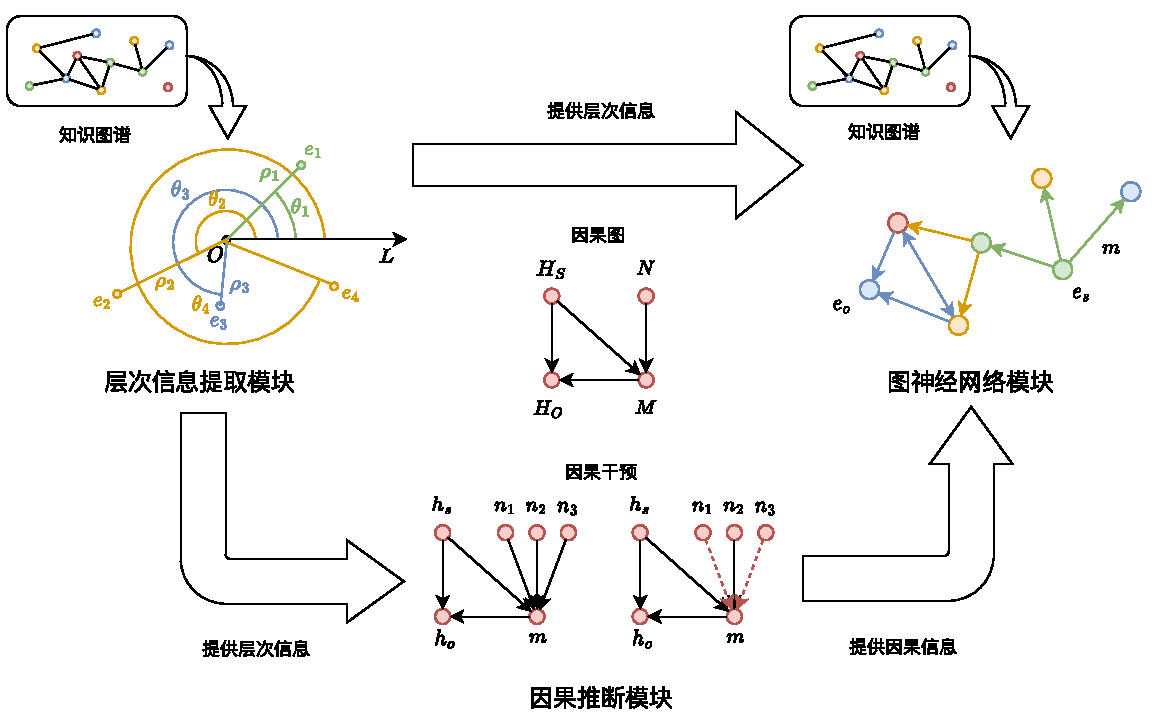
\includegraphics[width=0.9\textwidth]{2_NORMAN}
%   \caption{基于因果推断的知识图谱表示学习模型框架图}
%   \label{NORMAN}
% \end{figure}

\section{层次信息提取模块构建}
层次信息
% \begin{figure}
%   \centering
%   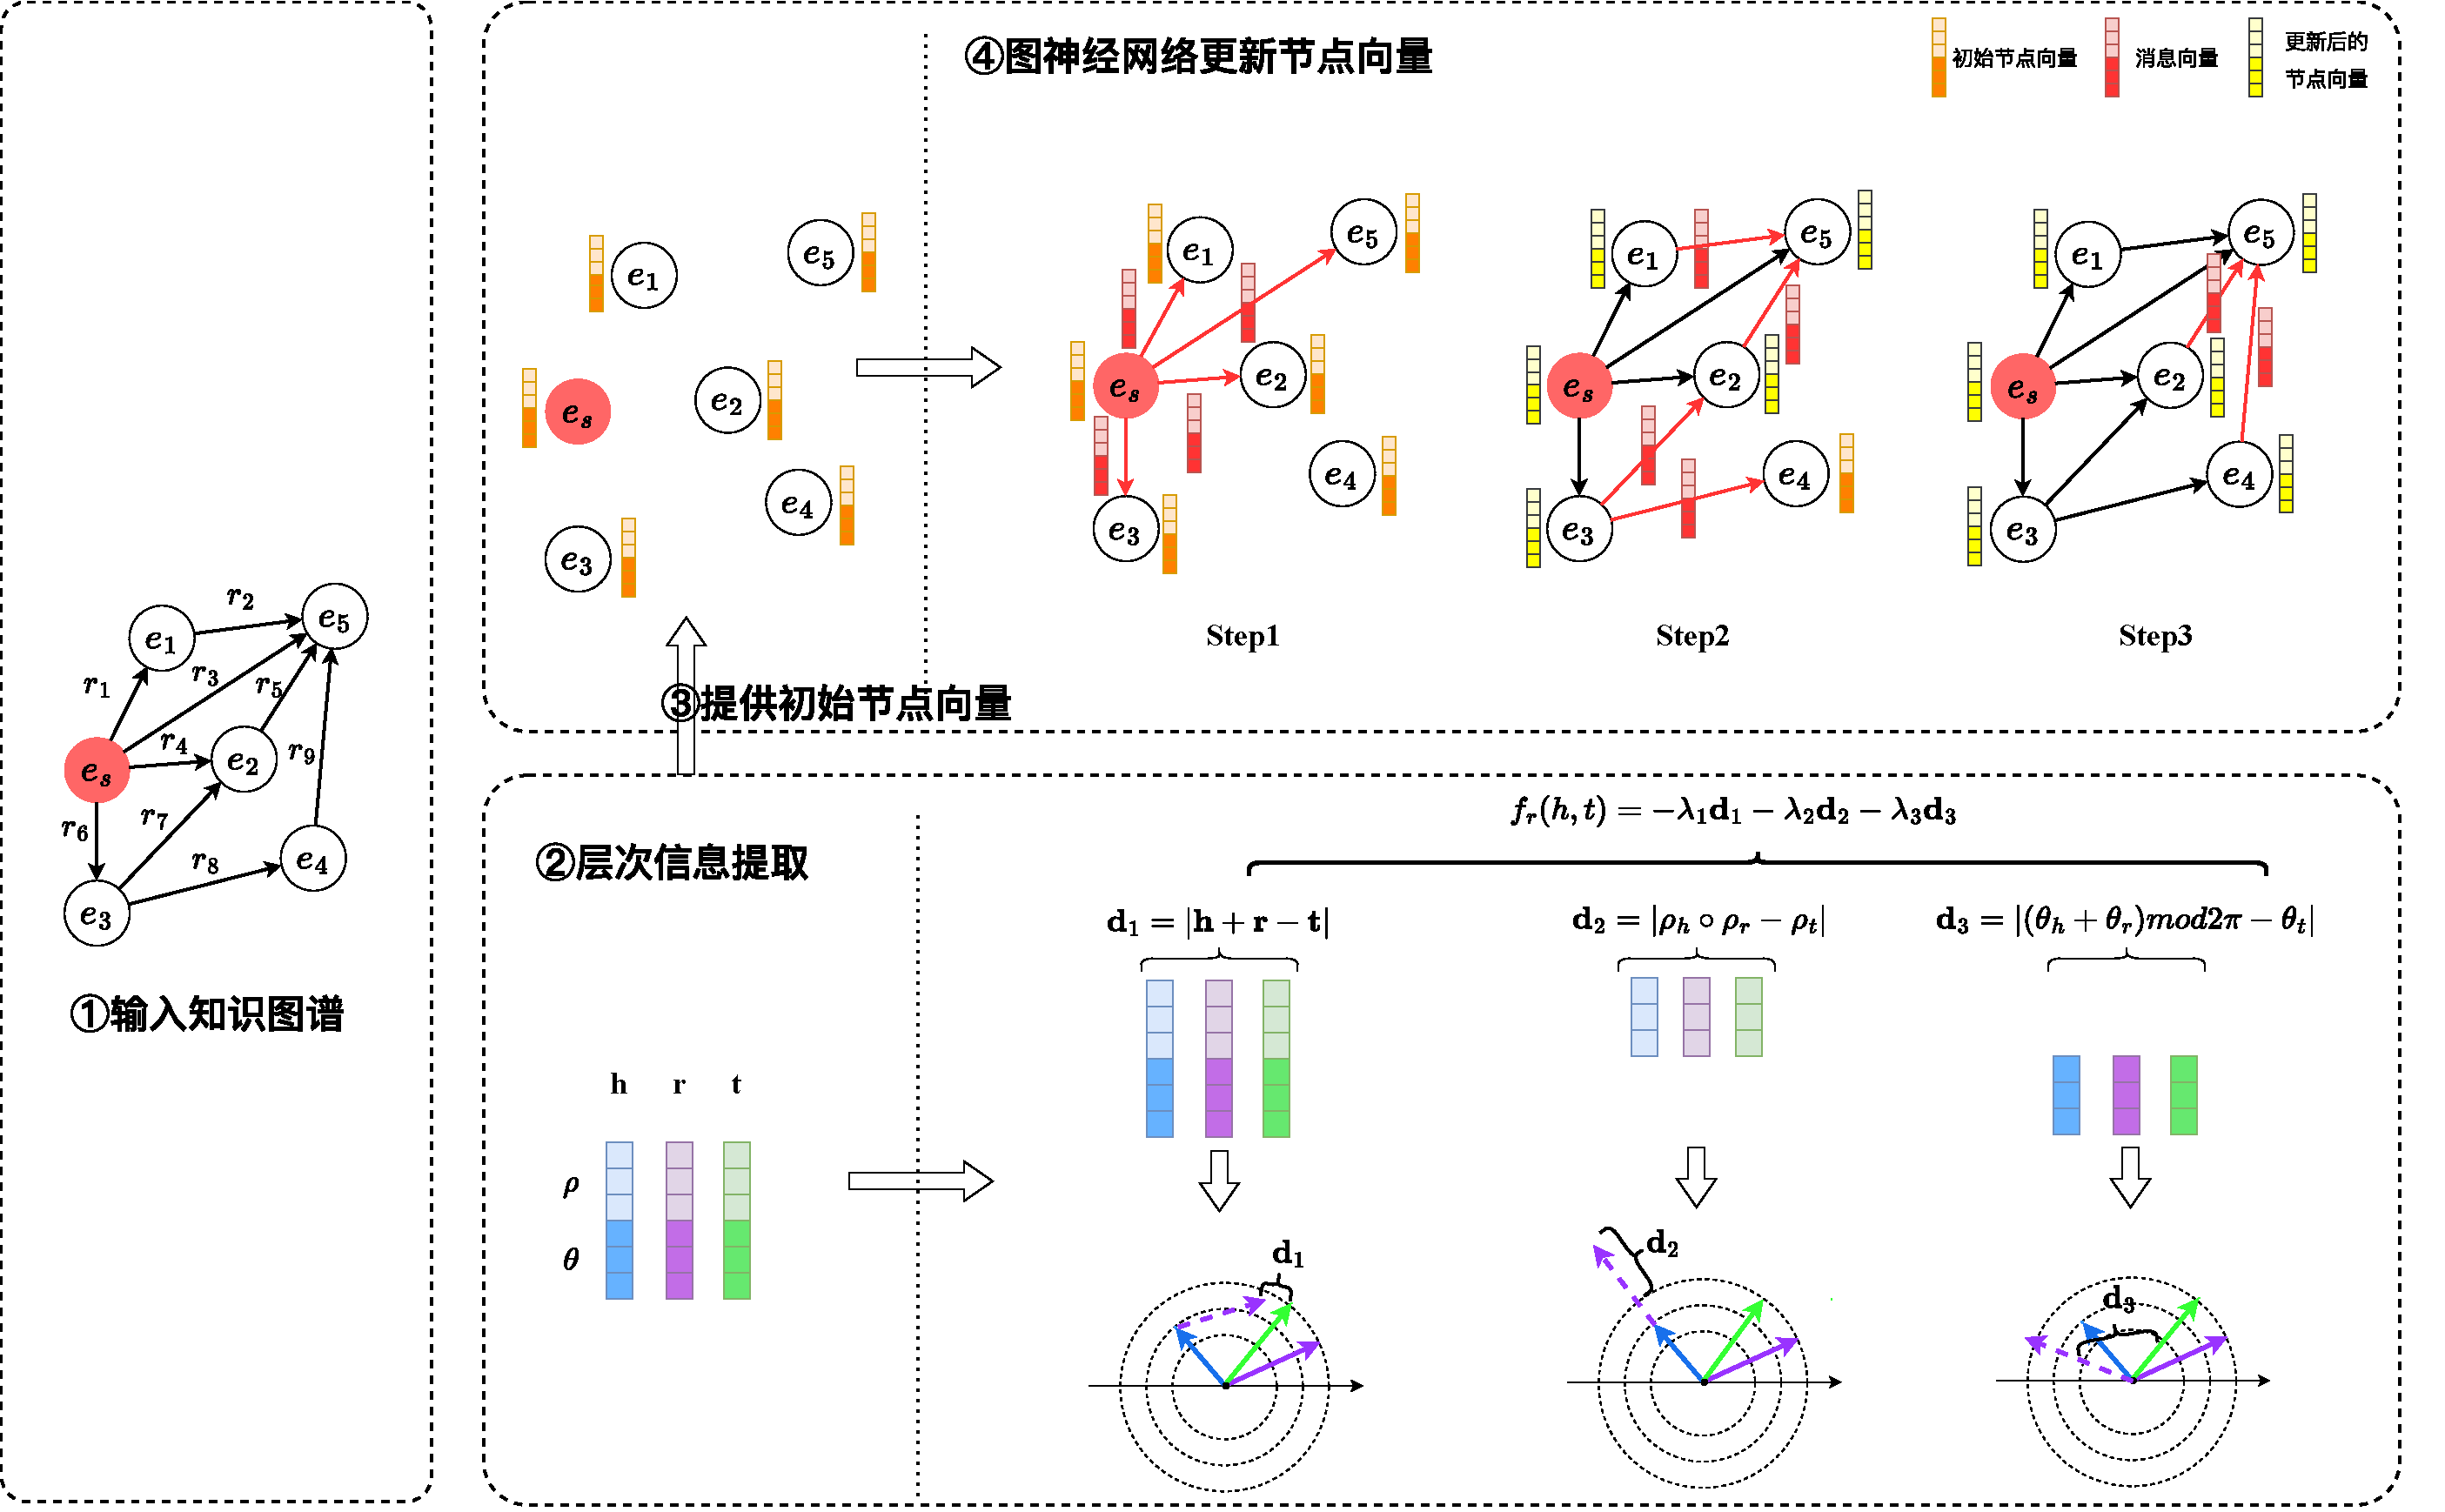
\includegraphics[width=0.9\textwidth]{2_Layers}
%   \caption{}
%   \label{Layers}
% \end{figure}

\section{因果推断模块构建}


\section{图神经网络模块构建}


\section{本章小结}
本章主要介绍了基于因果推断的知识图谱表示学习模型,该模型能够将结构化三元组知识信息转换成向量表示。模型首先通过层次信息提取模块将知识映射到极坐标系上,并通过聚类算法得到知识对应的层次信息。随后模型利用图神经网络模块,输入初始向量和知识层次信息,通过知识邻域信息传递进行数据更新,同时利用因果推断模块,根据因果不确定性、预测置信度和知识层次级别等多种因素,评估各个图神经网络节点是否接收特定邻域的信息。
本章首先给出了知识图谱表示学习任务的定义,随后给出了方法概览。最后详细介绍了本文提出的基于因果推断的知识图谱表示学习模型与策略。


\chapter{基于双重代理强化学习的知识推理模型}
本章提出一种基于双重代理强化学习的知识推理模型LAURA,该模型能够XXX。
本章包含六个部分:知识推理任务定义(2.1节),模型方法概览(2.2节),实体级强化学习模块构建(2.3节),层次级强化学习模块构建(2.4节),双重代理强化学习交互模块构建(2.5节),以及本章小结(2.6节)。

\section{知识推理任务定义}
知识推理任务的目标主要是基于现有知识,预测和推理新的知识的过程。根据知识推理步骤的长度,可以将知识推理方法分成两种,即单跳知识推理和多跳知识推理。
单跳知识推理的典型方法是直接通过知识图谱表示学习模型,采用链接预测的方式实现知识推理,即给定查询三元组$\left(h, r, ?\right)$或$\left(?, r, t\right)$,通过将知识图谱内所有关系或实体作为候选答案,输入到知识图谱表示学习模型中,从而将实体与关系映射到低维向量空间中,并通过得分函数进行打分,随后根据得分结果进行排序,选择得分最高的实体或关系作为答案,并完成知识推理。然而,上述单跳推理方法无法提供推理路径,这使得推理过程缺乏可解释性~\cite{wang2019deeppath}。
另一种推理方法,即多跳知识推理方法,能够利用知识图谱上的拓扑结构信息实现显式推理,并提供推理路径,因此具有更好的可解释性。多跳知识推理的典型方法是采用知识图谱表示学习和神经推理模型相结合的方式,首先获取知识图谱的初始表示,随后通过神经推理模型,从推理问题的初始实体开始,每次通过比较实体和邻域实体之间特定知识三元组的得分,获取得分最高的实体作为下一跳实体并进行后续推理,直到到达推理路径长度上限或到达目标实体为止。

本章涉及到的符号及定义如表XXX所示。

\section{基于双重代理强化学习的知识推理模型框架概览}
本章提出的DIANA模型能够结合知识图谱表示学习模型,通过强化学习框架,实现多粒度和高质量的知识推理。图XXX展示了该模型,模型主要包含三个模块,分别是实体级强化学习模块、层次级强化学习模块和双重代理强化学习交互模块。
对于实体级强化学习模块,该模块采用强化学习框架,在原始的实体知识图谱上,由一个智能体(agent)根据策略网络(policy network)选取动作空间中的动作(action),改变自身状态(state),当到达结束条件时根据任务完成情况得到奖励(reward)。完成训练后,模块可以对查询的知识进行推理,返回知识的推理路径和对应的置信度。
对于层次级强化学习模块,该模块采用与实体级强化学习模块相同的强化学习框架,区别在于该模块使用的是层次知识图谱。首先利用知识图谱表示学习模型中的层次信息提取模块获取各个实体对应的层级,并将位于相同层级的全部实体作为层级节点,不同层级间则根据是否存在至少一条实体关联构建层级关联,从而完成层次知识图谱构建。随后可以在层次知识图谱上训练层次级强化学习模型。完成训练后,模块可以对给定知识进行推理,并返回层级级别的知识推理路径和对应置信度。
对于双重代理强化学习交互模块,该模块为知识推理模型的核心模块,用于协调两个强化学习模块,实现模块间的信息交互。模块设计了协作策略网络和轨迹相似度奖励两部分内容。协作策略网络是对模块策略网络的扩展,除了考虑自身模块当前状态、历史状态之外,还将另一个模块的历史状态纳入决策过程。轨迹相似度奖励是对模块奖励的扩展,除了考虑自身模块的奖励,还将两个模块的历史动作轨迹分别进行编码,并计算相似度得分作为补充奖励。完成训练后,模块可以在实体级和层次级两个级别进行知识推理,并将结果进行整合,返回置信度高于阈值的知识推理路径和对应的置信度信息。
% \begin{figure}
%   \centering
%   \includegraphics[width=0.9\textwidth]{3_DIANA}
%   \caption{基于双重代理强化学习的知识推理模型框架图}
%   \label{DIANA}
% \end{figure}

\section{实体级强化学习模块构建}


\section{层次级强化学习模块构建}


\section{双重代理强化学习交互模块构建}


\section{本章小结}
本章主要介绍了基于双重代理强化学习的知识推理模型,该模型能够结合知识图谱表示学习模型,根据给定的查询结构化三元组知识信息进行显式的知识推理,返回知识推理路径和对应置信度信息。
本章提出的模型能够在实体级和层次级两种粒度下进行知识推理,其中层次级知识推理主要根据宏观层面的信息进行知识推理,优势是能够更好地统合全局信息,实体级知识推理主要根据微观层面信息进行推理,优势是能够更好地处理局部细节信息。通过双重代理强化学习交互模块,主要使用协作策略网络和轨迹相似度奖励两种方法,能够将两种级别的强化学习模块进行整合,提高知识推理效果。
本章首先给出了知识推理任务的定义,随后介绍了方法概览,最后详细介绍了本文提出的基于双重代理强化学习的知识推理模型的模型与策略。


\chapter{实验评估}
本章对第二章提出的知识图谱表示学习方法和第三章提出的知识推理方法进行实验评估。
4.1节介绍了本文系统的实验环境。
4.2节介绍了知识图谱表示学习任务的实验与评估信息。
4.3节介绍了知识推理任务的实验与评估信息。

\section{实验环境}
本文提出的系统使用Python语言编写,版本为3.10.1,使用的深度学习框架为PyTorch,版本为1.13.1。
本文进行的所有实验都是在型号为AMAX G448-X3的服务器上完成的,服务器的具体参数包括:CPU型号为Xeon Sliver 4314,GPU型号为GeForce RTX 3090,系统内存为64G,系统硬盘为500G,操作系统版本为Ubuntu 22.04.1 LTS。

\section{知识图谱表示学习模型实验与评估}
知识图谱表示学习模型的目标是将实体和关系嵌入到低维向量空间中,同时保留原有知识图谱的结构信息和底层语义信息。
由于通常难以直接评价知识图谱表示学习模型的好坏,因此常用的方法是利用模型解决知识图谱下游任务来评估模型效果。本文使用链接预测任务进行模型评估,即给定不完整的查询三元组,要求根据知识图谱中已有的事实预测查询三元组中缺失的内容。
链接预测任务可以表示为补全查询三元组$\left(h, r, ?\right)$或$\left(?, r, t\right)$的问题,其中$?$表示待补全的内容,也可以称为待预测实体。
在测试过程中,对于测试数据集中的每个三元组$\left(h, r, t\right)$,首先将头部实体$h$或尾部实体$t$替换为每个候选实体,以创建一组候选三元组。随后使用得分函数$f_r\left(h, t\right)$计算所有候选三元组的得分,并按照降序对候选三元组进行排序。本文开展的实验遵循Bordes等人提出的实体链接实验设置~\cite{bordes2013translating},该设置中不会将任何知识图谱中存在的事实三元组纳入排名序列中,从而确保排名中的三元组都是新的三元组。最后根据结果三元组序列可以评估模型执行链接预测任务的效果。
链接预测任务中常用的评价指标包括平均排序MR(正确答案排名的平均值)、平均倒数排序MRR(正确答案排名倒数的平均值)以及Hits@K(正确答案在序列中排名位于前K的比例)等。
平均排序MR的计算方式是$\mathrm{MR}=\frac{1}{|\mathrm{S}|} \sum_{\mathrm{i}=1}^{|\mathrm{S}|} \mathrm{rank}_{\mathrm{i}}=\frac{1}{|\mathrm{S}|}\left(\mathrm{rank}_1+\mathrm{rank}_2+\cdots+\mathrm{rank}_{\mathrm{i}}\right)$,其中$|\mathrm{S}|$是结果三元组的数量,$\mathrm{rank}_{\mathrm{i}}$是第$i$个三元组在链接预测结果序列中的排名,也就是正确三元组在预测三元组序列中的排名。由此可见,平均排序MR的结果越小代表模型效果越好。
平均倒数排序MRR与平均排序MR较为类似,区别在于平均倒数排序是对排序结果的倒数进行求和,计算方式为$\operatorname{MRR}=\frac{1}{|\mathrm{S}|} \sum_{\mathrm{i}=1}^{|\mathrm{S}|} \frac{1}{\mathrm{rank}_{\mathrm{i}}}=\frac{1}{|\mathrm{S}|}\left(\frac{1}{\mathrm{rank}_1}+\frac{1}{\mathrm{rank}_2}+\cdots+\frac{1}{\mathrm{rank}_{\mathrm{i}}}\right)$。可以发现,MRR和MR具有相同的作用,都能够用于评估模型的链接预测效果,同时根据相关工作介绍~\cite{hoyt2022unified},MR在多个性能指标上比MRR的表现更差,一般情况下推荐使用MRR作为评价指标,而不推荐使用MR。因此,本文选择MRR评估模型效果。
Hits@K是指在链接预测结果序列中正确答案排名小于$K$的三元组的平均占比,计算方式为$\mathrm{Hits@K}=\frac{1}{|\mathrm{S}|} \sum_{\mathrm{i}=1}^{|\mathrm{S}|} \mathbb{I}\left(\operatorname{rank}_{\mathrm{i}} \leq \mathrm{K}\right)$,其中$S$是三元组总数,$K$是目标排名范围,$\mathbb{I}\left(\cdot\right)$是指示函数,即若括号中的条件为真则其函数值为1,否则为0。一般情况下,取$K$为1、3和10。可以直观地发现,Hits@K的指标越大表明模型在链接预测任务上的效果越好。
综上所述,本文选择平均倒数排序MRR和Hits@K作为评价指标,评估模型在链接预测任务上的效果。

本节首先介绍了知识图谱表示学习模型的评估实验内容,即通过链接预测任务,评估模型的效果。随后介绍了任务的评价指标、实体链接数据集和具体的实验设置,并在最后比较本文提出的NORMAN模型和其他基线知识图谱表示学习模型在链接预测任务上的效果,进而对NORMAN模型的优势和劣势进行客观评估。

\subsection{数据集}
本文采用的数据集包括:FB15K-237~\cite{toutanova2015representing}、WN18RR~\cite{dettmers2018convolutional}和NELL-995~\cite{xiong2017deeppath}。上述三个数据集分别是从大规模知识图谱Freebase~\cite{bollacker2008freebase}、WordNet~\cite{glorot2010understanding}和NELL~\cite{carlson2010toward}采样得到的。
FB15K-237数据集在对Freebase知识图谱进行采样时删除了逆向关系,同时保留了其中的对称、反对称和组合关系。因此在FB15K-237数据集上的链接预测任务主要考察模型对上述三种关系的表达能力。在数据数量上,FB15K-237包含14541种实体和237种关系,同时包含了310116条三元组数据,数据量较大,需要模型能够处理大规模知识图谱数据。
WN18RR与FB15K-237类似,也是在对WordNet知识图谱进行采样时删除了逆向关系并保留了对称、反对称和组合关系,因此也是主要考察模型对上述三种关系的表达能力。WN18RR包含40943种实体和11种关系,并提供了93003条三元组数据,可以发现WN18RR的实体种类非常多,同时三元组数量较少,意味着每种实体对应的三元组数量较少,这增加了训练模型的难度。
NELL-995是从大规模知识图谱NELL中采样得到的数据集,保留了数量排名在前200名的关系对应的三元组数据。与FB15K-237和WN18RR不同的是,NELL-995保留了逆向关系,原因是该数据集是可以用于评估多跳知识推理问题的数据集,为了进行双向推理保留了双向边,因此NELL-995除了对称、反对称和组合关系外,还可以考察模型对逆向关系的表达能力。在数据数量上,NELL-995包含75492种实体和200种关系,并提供了154213条三元组。可以发现,NELL-995提供了较多的数据,需要模型有处理大规模知识图谱的能力。
实验采用的三种链接预测数据集的具体统计信息如表~\ref{Datasets1}所示。根据上述分析可知,三种数据集具有不同的特点,能够用于客观评估知识图谱表示学习模型的表示效果。

\begin{table}
  \centering
  \begin{tabular*}{0.95\textwidth}{@{\extracolsep{\fill}}lccccc}
		\toprule[1pt]
    数据集 & 实体数量 & 关系数量 & 训练集数量 & 验证集数量 & 测试集数量 \\ \hline
    FB15K-237 & 14541 & 237 & 272115 & 17535 & 20466\\
    WN18RR & 40943 & 11 & 86835 & 3034 & 3134\\
    NELL-995 & 75492 & 200 & 138793 & 7710 & 7710\\
		\bottomrule[1pt]
	\end{tabular*}
  \caption{链接预测数据集统计信息}
  \label{Datasets1}
\end{table}

\subsection{实验设置}


\subsection{实验结果与分析}


\section{知识推理模型实验与评估}
知识推理模型的目标是基于现有知识,预测和推理新的知识,并通过将新的知识补充到知识图谱上降低知识图谱的稀疏性,实现知识图谱补全。
为了评估知识推理模型的效果,我们选择了单跳知识推理和多跳知识推理两种实验来进行模型评估。
单跳知识推理任务和链接预测任务原理相同,通过将所有测试三元组$\left(h, r, t\right)$的头实体或尾实体替换为所有候选实体,得到一组候选三元组,随后调用知识推理模型评估候选三元组的得分,这里的获取得分有多种方法,可以是知识图谱表示学习模型的得分函数,也可以是强化学习等推理模型通过计算得到的置信度得分。最后按照得分的降序顺序对候选三元组进行排序,并根据结果三元组序列评估模型效果。
多跳知识推理任务则相对更加复杂一些,首先将测试三元组$\left(h, r, t\right)$的头实体或尾实体删除,得到对应查询三元组$\left(h, r, ?\right)$或$\left(?, r, t\right)$,随后要求模型根据已有的知识图谱进行查询,在指定跳数$T$的范围内进行推理,最后预测缺失的头实体或尾实体,将查询三元组进行补全,并对所有候选答案进行得分计算,同样是对得分进行降序排序,并根据最终排序结果评估模型效果。本文主要研究最大跳数$T$为4的多跳知识推理问题。
知识推理任务的评价指标同样为平均排序MR、平均倒数排序MRR和Hits@K等,根据知识图谱表示学习模型实验一节的分析,一般认为平均倒数排序MRR的表示能力优于平均排序MR,因此本文选择平均倒数排序MRR和Hits@K作为评估指标。
本节首先介绍了知识推理模型的评估实验内容,即通过链接预测任务,评估模型的效果。随后介绍了任务的评价指标、实体链接数据集和具体的实验设置,并在最后比较本文提出的NORMAN模型和其他基线知识图谱表示学习模型在链接预测任务上的效果,进而对NORMAN模型的优势和劣势进行客观评估。

\subsection{数据集}
本文在单跳知识推理和多跳知识推理两种任务上进行模型评估。
针对单跳知识推理任务,本文采用的数据集包括:FB15K-237、WN18RR和NELL-995。
另一方面,对于多跳知识推理任务,本文采用的数据集包括:FB15K-237-10\%、FB15K-237-20\%、FB15K-237-50\%、NELL23K和WD-singer~\cite{lv2020dynamic}。
在单跳知识推理任务中,由于单跳知识推理任务可以被理解为与链接预测任务相同,因此本文选择与知识图谱表示学习模型实验部分相同的数据集,即FB15K-237、WN18RR和NELL-995,从而能够更好的对本文提出的两种模型进行对比。
在多跳知识推理任务中,考虑到多条推理过程需要综合一定范围内的知识进行综合评估,为了测试本文提出的模型在不同稀疏程度的知识图谱上的性能,本文选择了多个基于FB15K-237数据集进行随机采样得到的数据集,即FB15K-237-10\%、FB15K-237-20\%和FB15K-237-50\%。由名字可以看出,这三个数据集分别随机保留了FB15K-237数据集的10\%、20\%和50\%的三元组数据,从而能够评估模型利用不同稀疏程度的知识图谱进行知识推理的能力。
此外,对于多跳推理任务,本文还选择了NELL23K和WD-singer这两个数据集。
NELL23K数据集是根据大规模知识图谱NELL中进行采样得到的数据集。具体而言,NELL23K提供了22925种实体和200种关系,同时提供了35358条三元组数据。可以看到,NELL23K的实体数据种类较多,同时三元组数量较少,这增加了训练模型的难度,需要模型根据实体种类以外的其他信息进行链接预测。
WD-singer数据集是从维基百科知识图谱Wikidata中采样的数据集,与上述其他数据集不同,WD-singer仅包含Wikidata中与歌手相关的内容,首先获取歌手相关的概念,随后通过这些概念获取对应的实体,构建实体列表。最后搜索包含实体列表中实体的三元组,形成最终数据集。WD-singer提供了10282种实体和135种关系,并提供了20508条三元组。可以发现WD-singer同样较为稀疏,可以考察模型对稀疏知识图谱的推理能力。
具体统计数量上,本部分采用的单跳推理测试数据集的统计数据见表~\ref{Datasets1},多跳推理测试数据集如表~\ref{Datasets2}所示。根据上文分析可知,本文选择的单跳和多跳知识推理数据集能够较好的评估模型的知识推理能力,同时能够评估模型在不同稀疏程度的知识图谱上的效果。

\begin{table}
  \centering
  \begin{tabular*}{0.95\textwidth}{@{\extracolsep{\fill}}lccccc}
		\toprule[1pt]
    数据集 & 实体数量 & 关系数量 & 训练集数量 & 验证集数量 & 测试集数量 \\ \hline
    FB15K-237-10\% & 11512 & 237 & 54887 & 3049 & 3049\\
    FB15K-237-20\% & 13166 & 237 & 82046 & 4558 & 4558\\
    FB15K-237-50\% & 14149 & 237 & 156448 & 8691 & 8691\\
    NELL23K & 22925 & 200 & 31822 & 1768 & 1768\\
    WD-singer & 10282 & 135 & 18458 & 1025 & 1025\\
		\bottomrule[1pt]
	\end{tabular*}
  \caption{多跳知识推理数据集统计信息}
  \label{Datasets2}
\end{table}

\subsection{实验设置}


\subsection{实验结果与分析}


\section{本章小结}



\chapter{总结与展望}
本章主要对本文的工作进行总结,并分析当前工作的优势与不足,最后提出未来工作的展望。

\section{主要工作总结}
本文的工作主要包括以下几个方面:

\section{未来工作展望}
尽管本文实现了XXX,但其中仍然存在一些不足之处。
本文的工作可以在以下几个方面进行改进:


\acknowledgement
测试

\thesisbib{paper}

% \thesisbib{paper}  % 该命令用于生成参考文献,采用 BIBTEX 工具自动生成。为此,需提供.bib 数据库文件名称作为该命令的参数,不需要包含扩展名。
% \bibliographystyle{seuthesix}
% \bibliographystyle{unsrt}
% \bibliography{paper}


\appendix
\resume{作者简介}
我是一个人

\end{document}
